\chapter{Introduction}

\section{Ultrafast Dynamics in Condensed Matter Systems}

timescales and processes in solids

\section{Attosecond Transient Absorption Spectroscopy (ATAS)}

\subsubsection{why are you doing it with HHG?}

include figure of pulse duration vs photon energy, showing different light sources (synchrotrons, HHG sources, XFEL, etc.) tie this into the timescales neccessary to probe condensed matter physics.

\subsection{overview of the technique}

references \cite{ramaseshaRealTimeProbingElectron2016}

The basic concept of an \textit{attosecond transient absorption spectroscopy} (ATAS) experiment is shown in \cref{fig:ATAS_Cartoon_Si_Leone}. In this experiment, a sample is placed at the combined XUV/IR focus in a transmission (normal) geometry. An XUV photon spectrometer is placed behind the sample and the transmitted XUV spectrum $S$ is measured as a function of XUV-IR delay. The IR light is not measured by the spectrometer.

Fundamentally, changes in photoabsorption correspond to electron and phonon dynamics in the sample. In condensed matter materials, these processes occur on the picosecond ($10^{-12}$ s), femtosecond ($10^{-15}$ s) and even attosecond ($10^{-18}$ s) time scales \cite{schultzeAttosecondBandgapDynamics2014,cushingDifferentiatingPhotoexcitedCarrier2019,zurchDirectSimultaneousObservation2017,volkovAttosecondScreeningDynamics2019}. At XUV energies, photons drive electronic transitions from a core-level state to one near the Fermi level, which requires electron population in the initial state and a vacancy in the final state. Because the initial state is tens or even hundreds of eV below the bandgap, it is shielded from the external IR field. The final states, being closer to the Fermi level, enjoy no such shielding. Therefore they can be distorted by the external IR field, and the electron population can be transferred between these states in response to the IR field. After an initial IR excitation, electrons relax via different scattering channels, including with other electrons or phonon modes with longer lifetimes. Provided the dipole selection rules allow it, the photoabsorption spectrum is sensitive to all of these dynamics. Thus by measuring the XUV spectrum as a function of XUV-IR delay, we can track the electronic and phononic response of a sample to an ultrafast IR excitation.


\subsubsection{induced dipole interpretation}

\subsubsection{population transfer and probing interpretation}

\subsubsection{comparison of absorptive and reflective measurements}


\begin{figure}
	\centering
	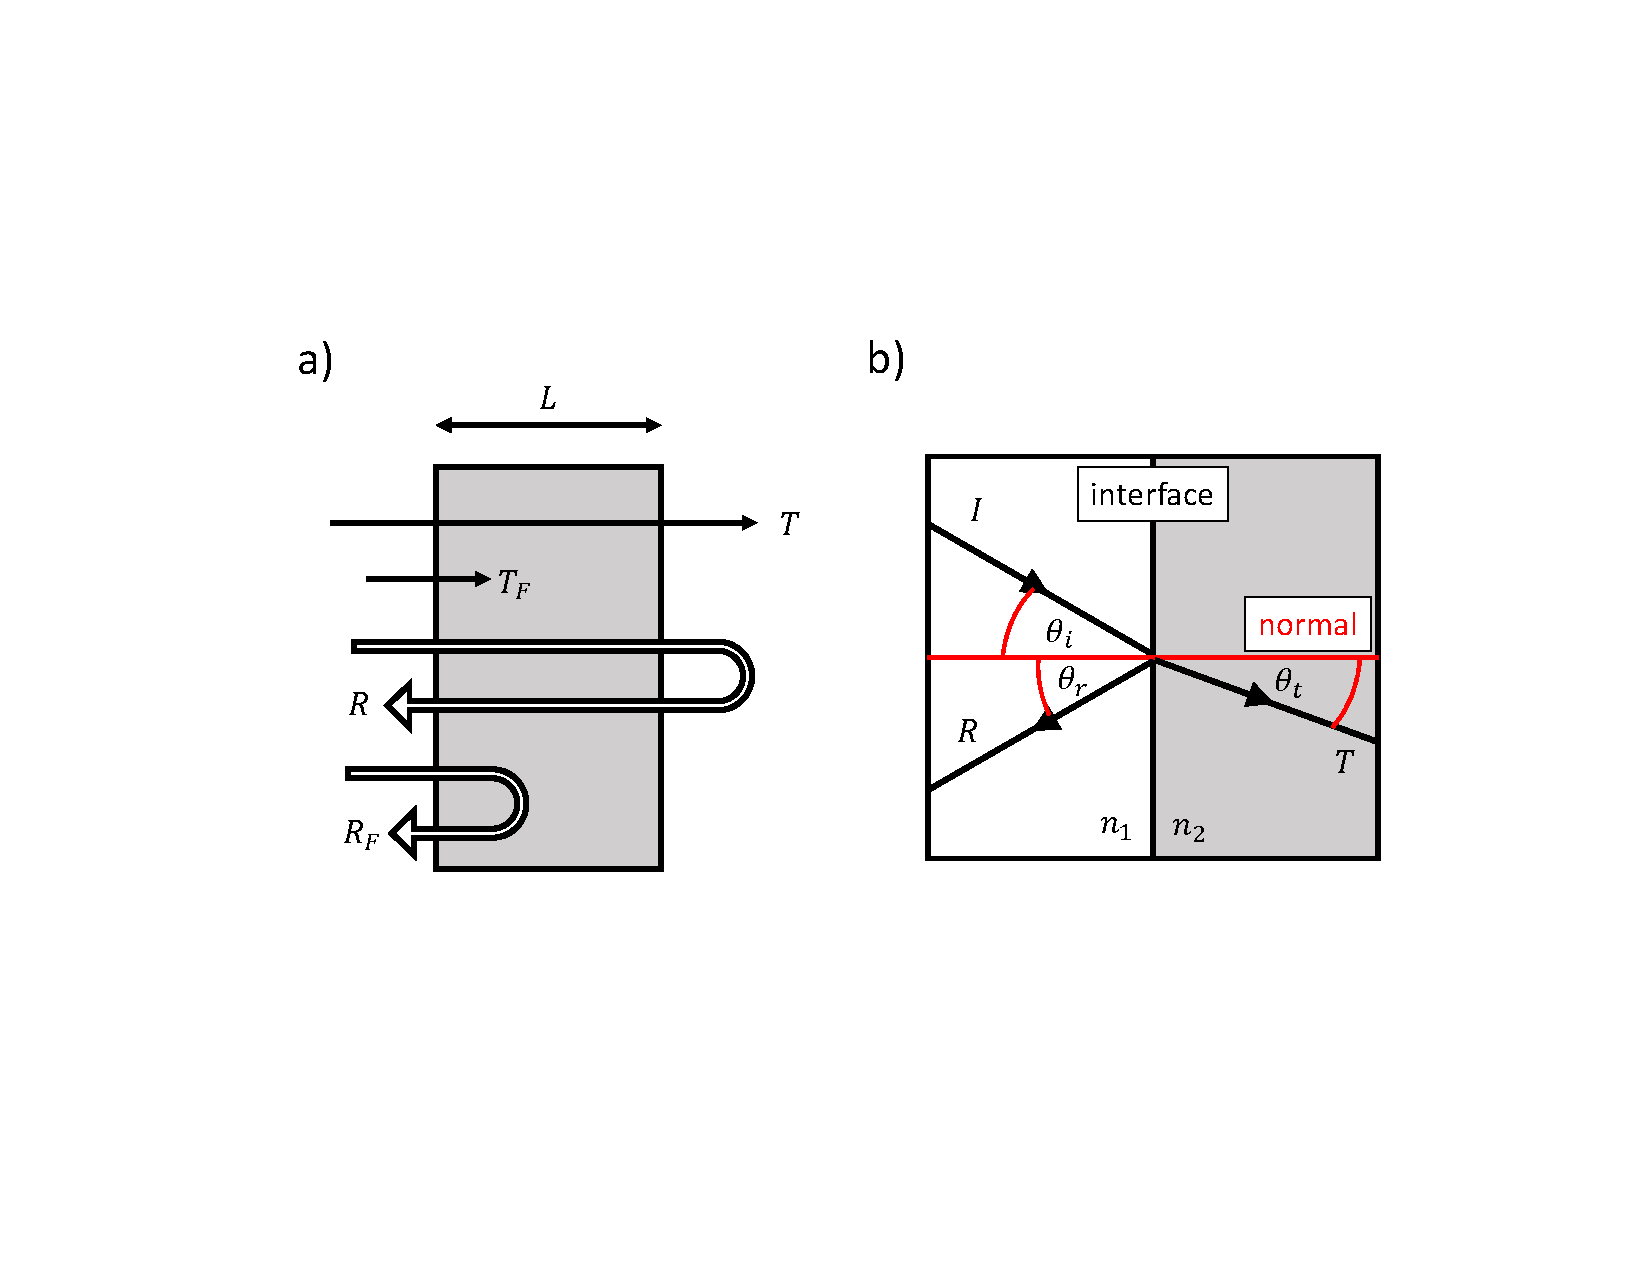
\includegraphics[width=0.75\textwidth]{figures/chap1/Fresnel_Geometry.pdf}
	\caption{Normal and non-normal incident geometries. \textbf{a)} Normal incidence geometry showing Fresnel coefficients $R_F$, $T_F$ for interfaces and total transmission $T$ and reflectance $R$ for a slab of thickness $L$. Figure recreated from \cite{nichelattiComplexRefractiveIndex2002}. \textbf{b)} Non-normal geometry showing definitions of angles $\theta_i, \theta_r$ and $\theta_t$ with respect to each interface.}
	\label{fig:Fresnel_Geometry}
\end{figure}

In a transient absorption experiment, we measure the transmission $T$ of a sample in response to excitation by an external field. Generally speaking, $T$ depends on both parts of the complex refractive index: $\tilde{n} = n + i k$. However, in a normal transmission geometry it turns out that the contribution of $\Im(\tilde{n})$ dominates the measured signal, and to a good approximation the role of $\Re(\tilde{n})$ can be ignored. Note that in a non-normal reflection geometry, both parts of $\tilde{n}$ make significant contributitions to the measured signal. In the following discussion we will analyze the Fresnel equations to see why this is the case. This section will draw from arguments made in reference \cite{nichelattiComplexRefractiveIndex2002}.

First, we consider the normal geometry shown in the left panel of \cref{fig:Fresnel_Geometry}. We write the complex index of refraction in the following form:
\begin{equation}
\begin{aligned}
\tilde{n} &= n - i k \\
&= (1-\delta) - i \beta
\end{aligned}
\label{eqn:complex_index}
\end{equation}
The Fresnel coefficients $R_F$ and $T_F$ describe the interface reflectance and transmittance and depend on both parts of the complex index $\tilde{n}$. For normal incidence, they are:
\begin{equation}
\begin{aligned}
R_F &= \left| \frac{n-ik-1}{n-ik+1}   \right|^2 \\
T_F &=  \frac{4n}{\left|n-ik+1\right|^2}
\end{aligned}
\label{eqn:fresnel_normal}
\end{equation}
Absorption in the bulk is described via the absorption length $\alpha$:
\begin{equation}
\alpha = 4 \pi k / \lambda
\end{equation}
Ignoring interface effects, the transmisison through the bulk is:
\begin{equation}
T_{\text{bulk}} = \exp( - \alpha L)
\end{equation}
Note that $\alpha$ and $T_{\text{bulk}}$ only depend on $k$.

The total reflectance $R$ and transmission $T$ are the result of interface effects plus bulk effects. We must consider the case where the detected light is the result of multiple reflections within the sample. Neglecting interference, we consider the case of $2N$ bounces where the laser's coherence length is less than the thickness of the bulk. In this case, the sum is incoherent with the expressions for $T$ and $R$ given by:
\begin{equation}
\begin{aligned}
R &= R_F + R_F T_F^2 T_{\text{bulk}}^2 \sum_{m=0}^{N} \left[ R_F T_{\text{bulk}} \right]^{2m} \\
T &= T_F^2 T_{\text{bulk}} \sum_{m=0}^{N} \left[ R_F T_{\text{bulk}} \right]^{2m}
\end{aligned}
\label{eqn:Fresnel_coefs_N_bounce}
\end{equation}
For the case of an infinite number of bounces, \cref{eqn:Fresnel_coefs_N_bounce} simplifies to:
\begin{equation}
\begin{aligned}
R &= R_F + \frac{R_F T_F^2 T_{\text{bulk}}^2}{1-R_F^2 T_{\text{bulk}}^2} \\
T &= \frac{T_F^2 T_{\text{bulk}}}{1-R_F^2 T_{\text{bulk}}^2},
\end{aligned}
\label{eqn:Fresnel_coefs_inf_bounce}
\end{equation}
whereas if only a single bounce occurs, \cref{eqn:Fresnel_coefs_N_bounce} reduces to:
\begin{equation}
\begin{aligned}
R &= R_F + R_F T_F^2 T_{\text{bulk}}^2 \\
T &= T_F^2 T_{\text{bulk}}
\end{aligned}
\label{eqn:Fresnel_coefs_1_bounce}
\end{equation}

We now consider the fractional error introduced by ignoring the interface effects described by $T_F$ and $R_F$. That is, what would happen if we assume that the interfaces have no effect on the transmitted intensity? We introduce the relative error $\epsilon$ made by ignoring the Fresnel coefficients of \cref{eqn:Fresnel_coefs_inf_bounce}:
\begin{equation}
\epsilon \equiv \frac{T_{\text{bulk}}}{T} - 1
\label{eqn:Fresnel_rel_err}
\end{equation}

\begin{figure}
	\centering
	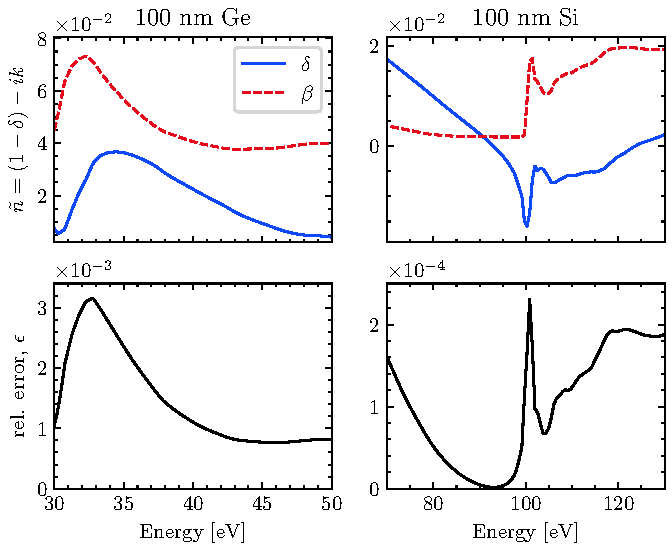
\includegraphics[width=0.9\textwidth]{figures/chap1/Ge_Si_transmission_Fresnel.pdf}
	\caption{Consequences of ignoring the real part of $\tilde{n}$ when calculating the transmission $T$ of germanium (left) and silicon (right). Top panels: complex refractive index. The Ge $M$-edge absorption feature is visible near 30-35 eV, and the Si $L$-edge is near 100 eV. Data from \cite{gulliksonCXROXRayInteractions}. Bottom panels: relative error in $T$, as defined in \cref{eqn:Fresnel_rel_err}, introduced by ignoring the contribution of $\Re(\tilde{n})$. An infinite number of bounces (\cref{eqn:Fresnel_coefs_inf_bounce}) is assumed.}
	\label{fig:Ge_Si_transmission_Fresnel}
	% plotted using \Python Scripts\CXRO\test\real_imag_index_plotting.py
\end{figure}

As an example, consider a 100 nm thick Ge sample measured in transmission near the Ge $M$-edge (about 30 eV), as shown in \cref{fig:Ge_Si_transmission_Fresnel}. The relative error is in the range of a few parts in $10^3$, well below our experimental detection limit. Silicon was chosen due to its data availability above and below the absorption edge, but this behavior should hold for all materials in normal transmission.

The real part of the complex index becomes important when the sample isn't normal to the beam, as shown in the right panel of \cref{fig:Fresnel_Geometry}. In this case, the Fresnel equations are a bit messier:
\begin{equation}
\begin{aligned}
R_s &= \left| \frac{\tilde{n}_1 \cos \theta_i - \tilde{n}_2 \cos \theta_t}{\tilde{n}_1 \cos \theta_i + \tilde{n}_2 \cos \theta_t}  \right|^2 \\
R_p &= \left| \frac{\tilde{n}_1 \cos \theta_t - \tilde{n}_2 \cos \theta_i}{\tilde{n}_1 \cos \theta_t + \tilde{n}_2 \cos \theta_i}  \right|^2 \\
T_s &= 1 - R_s \\
T_p &= 1 - R_p \\
%\theta_t &= \sqrt{1- \left( \frac{n_1}{n_2} \sin \theta_i \right)^2}
\end{aligned}
\label{eqn:Fresnel_nonnormal}
\end{equation}

Here, the subscripts $s$ and $p$ denote the polarization relative to the surface normal. For a sample in vacuum, $\tilde{n}_1=1$ and $\tilde{n}_2$ is the index of the sample. We can extract the relevant physics without any additional manipulation of \cref{eqn:Fresnel_nonnormal}. Right away, we can see that unlike \cref{eqn:fresnel_normal}, \cref{eqn:Fresnel_nonnormal} is symmetric in the real and imaginary parts of the sample's complex index, $\tilde{n}_2$. In the limit of a thick slab, ($L \gg \alpha$), the light is attenuated before it can reflect off the back surface and we have $T \rightarrow 0$ and $R \rightarrow R_{s,p}$. That is, the only contributions to the reflected intensity are from the interface and possibly the sample volume within $z \approx 1/\alpha$ of the interface. As a result, both parts of $\tilde{n}_2$ will make significant contributions to the reflected intensity. This geometry is common in transient reflection-absorption experiments \cite{cirriAchievingSurfaceSensitivity2017,kaplanFemtosecondTrackingCarrier2018}.



complex refractive index

sample requirements and preparation

pointing stability (in reflection, sample is an XUV optic)

\subsection{previous work}
what is state of the art?

previous work in condensed matter (Si, Ge, Si-Ge, etc)

motivation for long-wavelength studies in condensed matter

\subsection{physical observables in ATAS}
limited k-space information (requires single crystal)

transmission geometry measures imaginary and not the real part of n

\subsection{interpretation of experimental data}

absorbance $A$:

\begin{equation}
A(E) = - \log_{10} (T) = -\log_{10} \left( \frac{S_{\textrm{gs}}(E)}{ S_{\textrm{vac}} (E)} \right)
\label{eqn:absorbance}
\end{equation}

change in absorbance $\Delta A$:

\begin{align}
\Delta A (E, \tau) &= A_{\textrm{sig}}(E,\tau) - A_{\textrm{gs}} (E) \nonumber \\
&= -\log_{10} \left( \frac{S_{\textrm{sig}}(E, \tau)}{ S_{\textrm{vac}} (E)} \right) -\log_{10} \left( \frac{S_{\textrm{gs}}(E)}{ S_{\textrm{vac}} (E)} \right) \nonumber \\
&= -\log_{10} \left( \frac{S_{\textrm{sig}} (E, \tau)}{ S_{\textrm{gs}} (E)} \right)
\end{align}

\section{High Harmonic Generation}

\label{sec:HHG}

High harmonic generation (HHG) is the extremely nonlinear process in which a strong infrared field produces light with frequencies that are integer multiples of the fundamental field after interacting with a medium. Rather than providing a first principles discussion of HHG, the main objective of this section is to understand how we can produce bright attosecond XUV light pulses with a sufficient spectral coverage for use in an ATAS experiment.


We consider the case of an atom in strong laser field, where the electric field of the laser is comparable to the Coulomb field of the parent atom. Under these conditions, there is an appreciable chance of ionization. To determine which physical process is responsible for the ionization, we must consider two energy scales: the ionization potential of the atom $I_p$ and the ponderomotive energy $U_p$:
\begin{equation}
U_p = \frac{q_e^2 F_0^2}{4 m_e \omega^2} \propto I_0 \lambda^2
\label{eqn:Up}
\end{equation}
where $m_e$ is the electron mass, $q_e$ is the electron charge, $\omega$ is the frequency, $F_0$ is the electric field strength, $I_0$ is the intensity, and $\lambda$ is the wavelength of the laser. A more useful form of \cref{eqn:Up} is given below:
\begin{equation}
U_p \textrm{ [eV]} = \left( 9.33738 \times 10^{-5} \right) \times I_0 \textrm{[PW/cm\textsuperscript{2}]} \times \lambda\textrm{[nm]}^2
\label{eqn:Up-numbers}
\end{equation}

The Keldysh parameter $\gamma$ compares the magnitudes of these two energy scales \cite{keldyshIonizationFieldStrong1965}:
\begin{equation}
\gamma = \sqrt{\frac{I_p}{2 U_p}}
\end{equation}
The value of $\gamma$ determines the physical mechanism responsible for ionization. When $\gamma \gg 1$, we are in the multi-photon ionization (MPI )regime; $\gamma \le 1/2$ corresponds to tunnel ionization, and $\gamma \ll 1$ corresponds to over the barrier (OTB) ionization. We will restrict our discussion to the tunnelling regime, where HHG occurs.

- spectral coverage of harmonics

- pulse duration of harmonic light

Gas phase HHG 

symmetry leads to odd harmonics.

gas and solid HHG has been studied

\subsection{Single Atom Response}

\label{sec:single-atom-response}

\begin{figure}
	\centering
	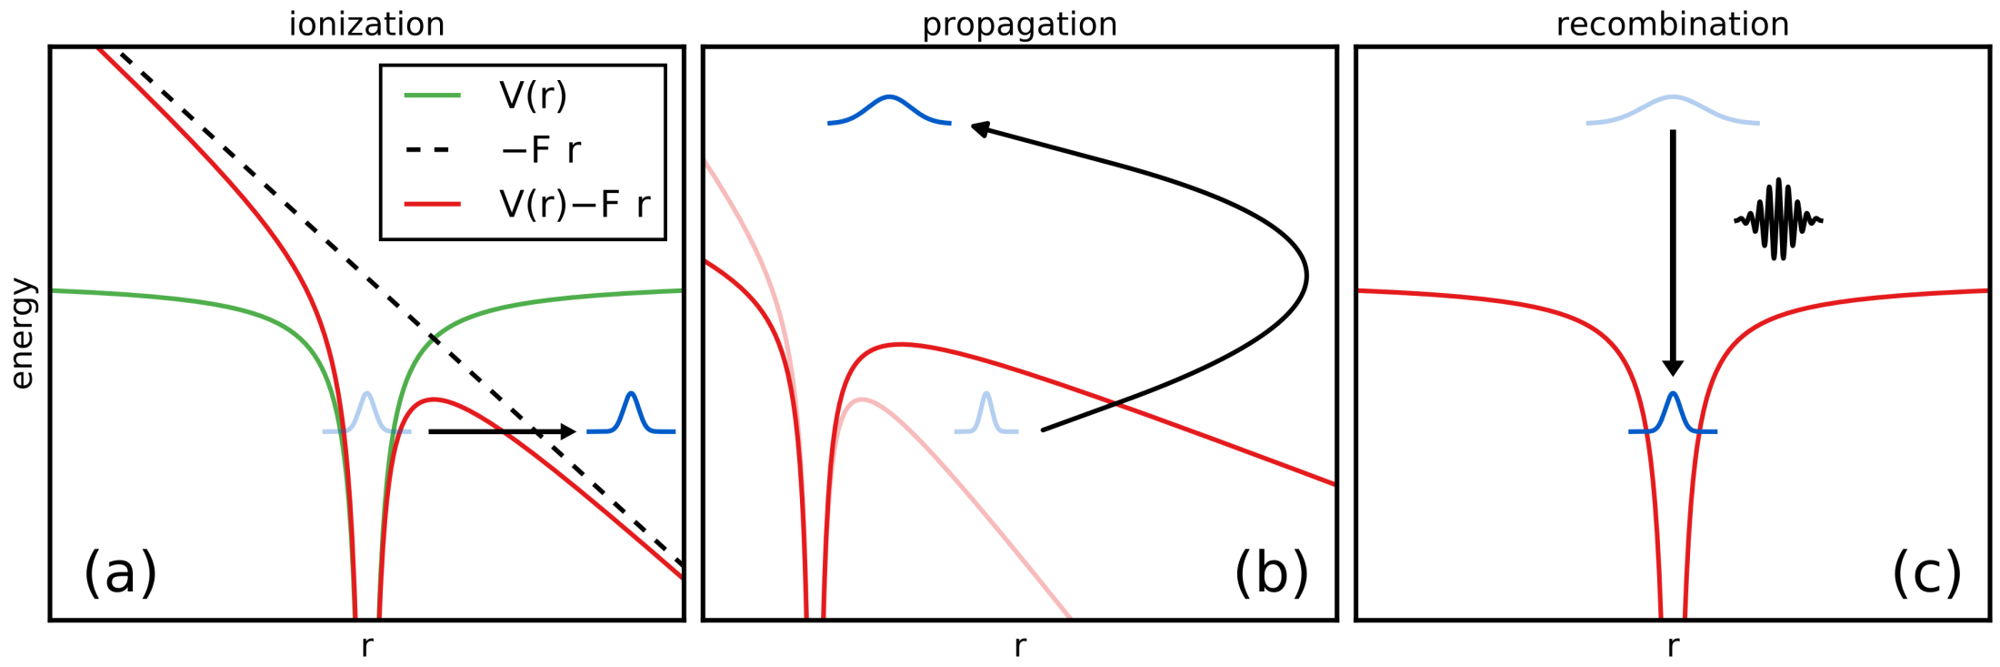
\includegraphics[width=0.75\textwidth]{figures/chap1/ThreeStepModel.png}
	\caption{The three step model of HHG. Figure adapted from \cite{schounAttosecondHighHarmonicSpectroscopy2015}.}
	\label{fig:ThreeStepModel}
\end{figure}

\begin{figure}
	\centering
	\subfloat[]{
		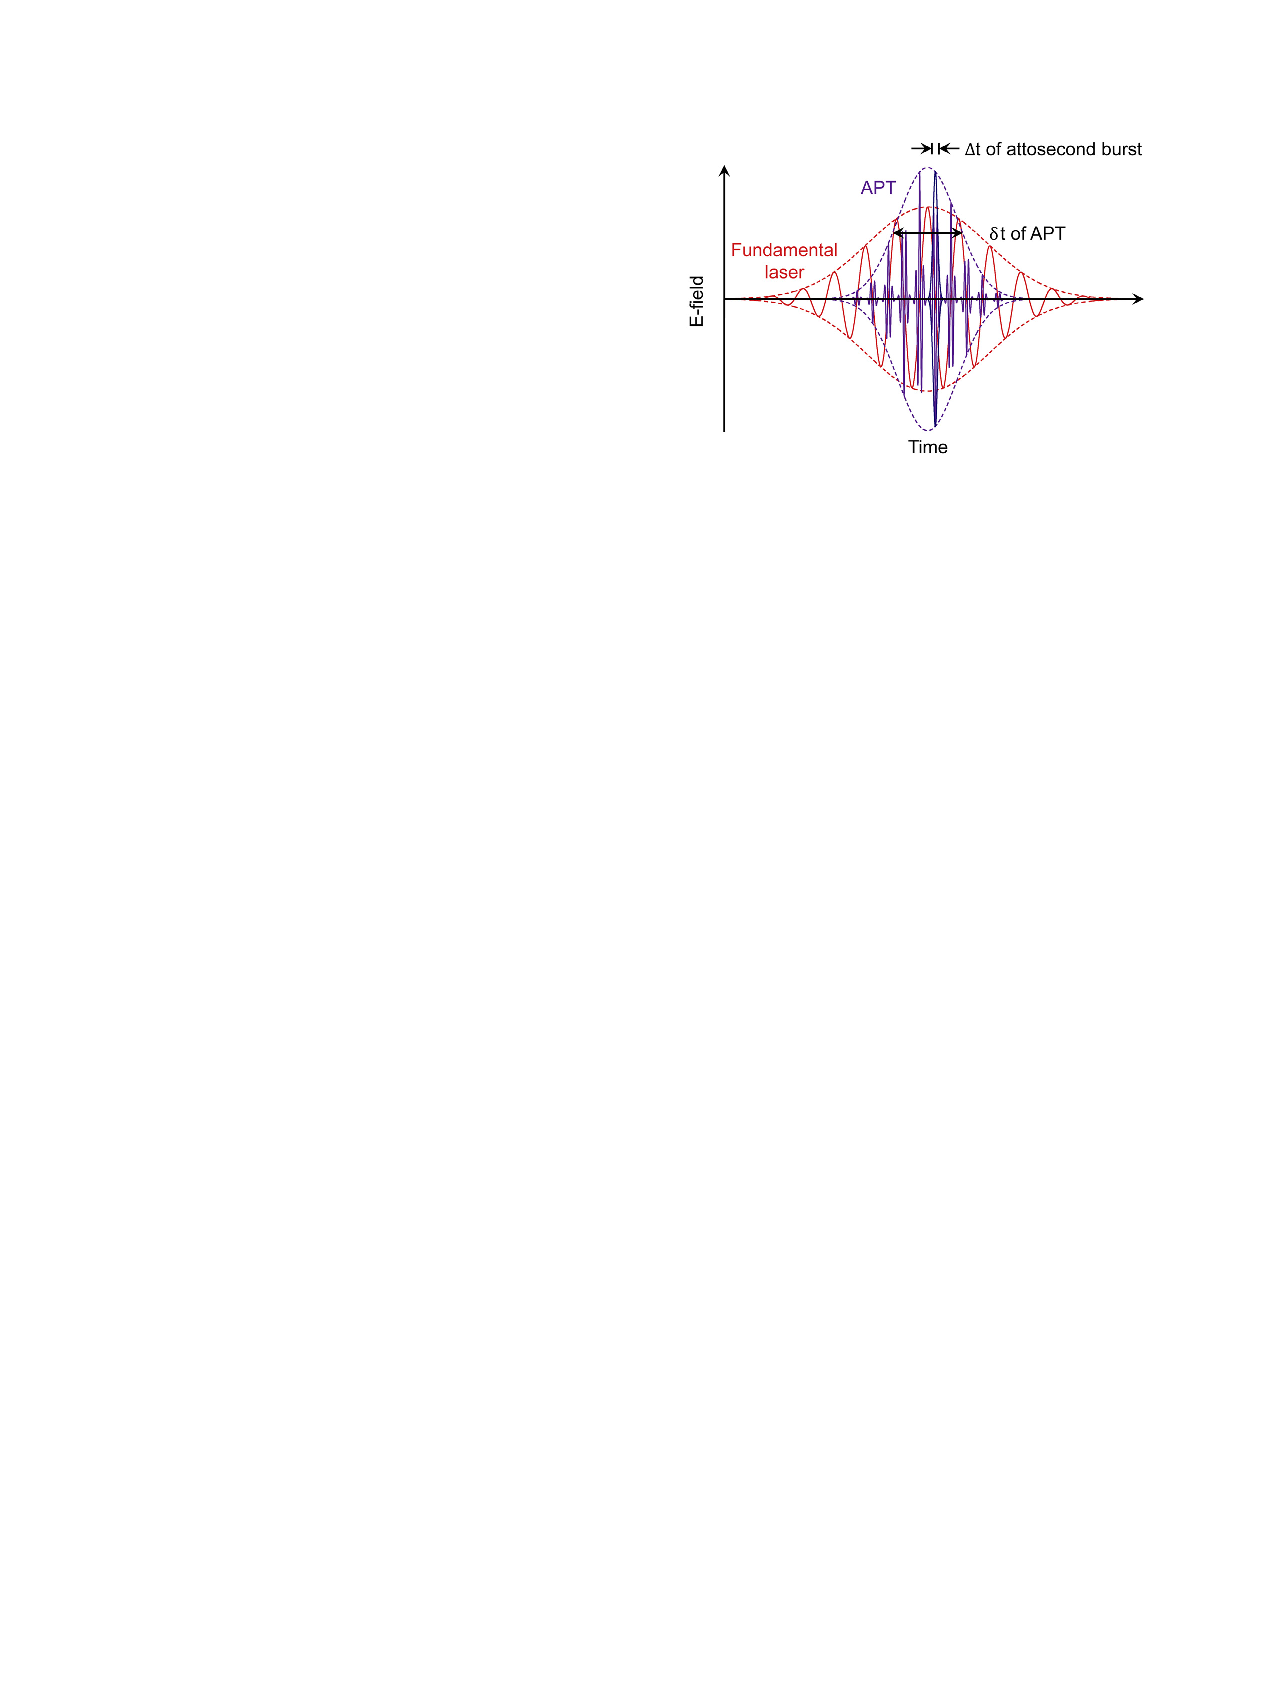
\includegraphics[width=0.4\textwidth]{figures/chap1/eich_APT_a.pdf}
		\label{fig:APT_time_domain}}
	\qquad
	\subfloat[]{
		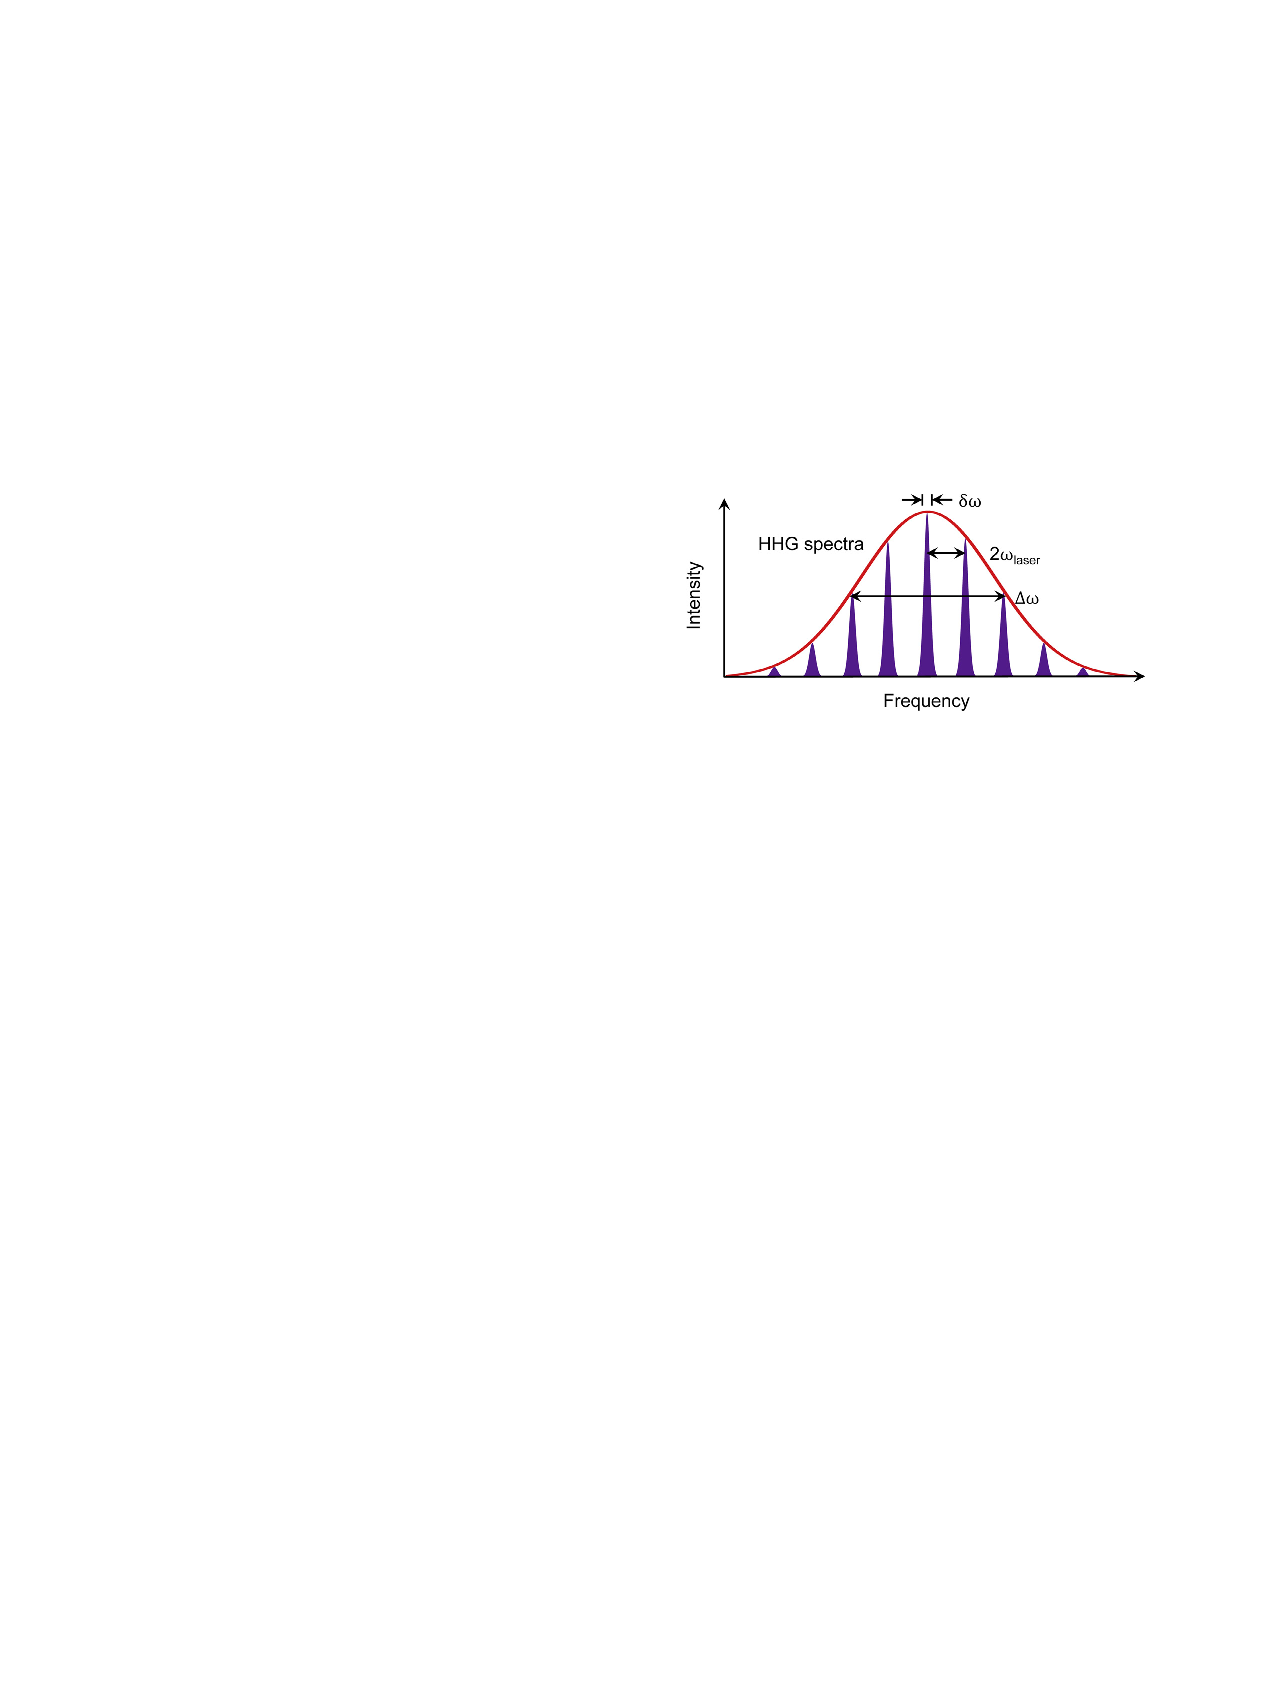
\includegraphics[width=0.4\textwidth]{figures/chap1/eich_APT_b.pdf}
		\label{fig:APT_freq_domain}}
	\caption{Time and frequency domain pictures of HHG. Figure adapted from \cite{eichTimeAngleresolvedPhotoemission2014}.}
	\label{fig:APT_IR_field}
\end{figure}

\begin{table}[]
	\centering
	\begin{tabular}{l|l|l|l|l|l|l|l|l}
		atom & $I_p$ {[}eV{]} & $I_p$ {[}at. u.{]} & $l$ & $m$ & $F_0$ {[}at. u.{]} & $F_b$ {[}at. u.{]} & $c_{n*l^*}^2$ & $f(l,m)$ \\ \hline
		He & 24.5874 & 0.90357 & 0 & 0 & 2.42946 & 0.20412 & 4.25575 & 1 \\
		Ne & 21.5645 & 0.792481 & 1 & 0 & 1.99547 & 0.15702 & 4.24355 & 3 \\
		Ar & 15.7596 & 0.579155 & 1 & 0 & 1.24665 & 0.08386 & 4.11564 & 3 \\
		Kr & 13.9996 & 0.514476 & 1 & 0 & 1.04375 & 0.06617 & 4.02548 & 3 \\
		Xe & 12.1298 & 0.445762 & 1 & 0 & 0.84187 & 0.04968 & 3.88241 & 3
	\end{tabular}
	\caption{ADK parameters.}
	\label{tab:ADK-params}
\end{table}

\begin{figure}
	\centering
	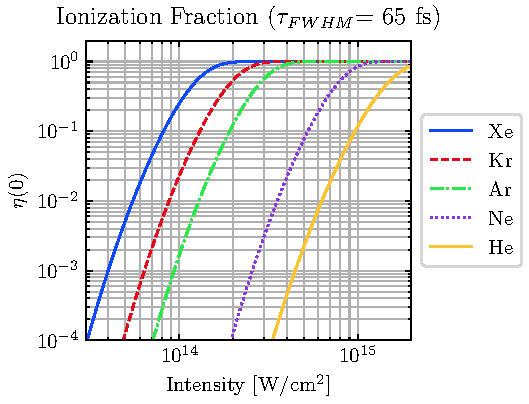
\includegraphics[width=0.75\textwidth]{figures/chap1/ADK_ion_frac_TL.pdf}
	\caption{Ionization fraction at the peak of a 65 fs pulse ($t=0$), calculated using the cycled-averaged OTB-corrected ADK rate.}
	\label{fig:ADK_ion_frac}
	% figure created in \Python Scripts\HHG_Phasematching-master\test\ADK_test_updated.py
\end{figure}

\begin{figure}
	\centering
	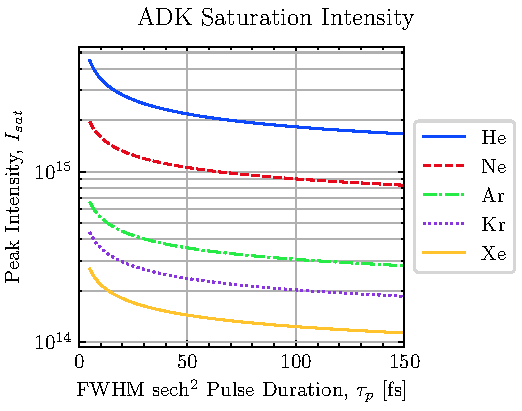
\includegraphics[width=0.75\textwidth]{figures/chap1/saturation_intensity.pdf}
	\caption{ADK saturation intensity for a sech$^2$ pulse.}
	\label{fig:saturation_intensity}
	% figure created in \Python Scripts\HHG_Phasematching-master\test\ADK_test_updated.py
\end{figure}

\begin{figure}
	\centering
	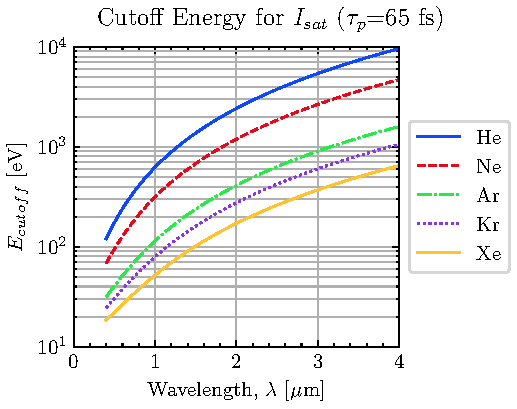
\includegraphics[width=0.75\textwidth]{figures/chap1/saturation_intensity_cutoff.pdf}
	\caption{High harmonic cutoff energy for a 65 fs FWHM pulse at saturation intensity.}
	\label{fig:saturation_intensity_cutoff}
	% figure created in \Python Scripts\HHG_Phasematching-master\test\ADK_test_updated.py
\end{figure}


We start with a microscopic picture of harmonic generation, focusing on the interaction between a single atom and the laser field. In the early 1990s, a semi-classical model was developed to describe the process of high harmonic generation in three discrete steps: tunnel ionization, classical propagation in the vacuum, and recombination of the electron and the parent ion \cite{schaferThresholdIonizationHigh1993,corkumPlasmaPerspectiveStrong1993}. This model accurately predicts many of the fundamental features of HHG.

\subsubsection{Strong Field Ionization}

In the three step model, the laser's electric field strength is on the order of the atomic potential that binds the electron to its parent atom. The valence electron's wavepacket evolves subject to the sum of the shielded Coloumb field and the spatially varying laser field. In this configuration, the electron can tunnel out of the distorted Coloumb field, as shown in the left panel of \cref{fig:ThreeStepModel}. This step is most likely to occur at the peak of the field, which occurs every half-cycle of the laser period.

The ionization rate from the ground state in the tunnelling regime is best described by an analytical formula first derived by Ammosov, Delone and Krainov in 1986 \cite{ammosovTunnelIonizationComplex1986,changFundamentalsAttosecondOptics2011,laiExperimentalInvestigationStrongfieldionization2017}. The resulting equation bears their names (ADK):

% these equations are from Lyte's thesis:
%\begin{equation}
%\omega(t) = \omega_p \left|C_{n*}\right|^2 \left(\frac{4 \omega_p}{\omega_t}\right)^{2 n*1-1} \exp \left(- \frac{4 \omega_p}{3 \omega_t}\right)
%\end{equation}
%with:
%\begin{align}
%\omega_p &= \frac{I_p}{\hbar} \\
%\omega_t &= \frac{e E(t)}{\sqrt{2 m I_p}} \\
%n^* &= Z \sqrt{\frac{I_H}{I_p}} \\
%\left|C_{n*}\right|^2 &= \frac{2^{2n*}}{n^* \Gamma (n^*+1) \Gamma (n^*)}
%\end{align}
%$I_p$ is the ionization potential of the atom, $E(t)$ is the electric field of the laser, $m$ is the electron mass, $Z$ is the ion charge after ionization, $I_H$ is the ionization potential of atomic hydrogen, and $\Gamma(x)$ is the gamma function.

%these equations are from Zenghu's book (p.183-4)} \cite{changFundamentalsAttosecondOptics2011}:
%$n^*$ is the effective prinicple quantum number, $l^* = n^* -1 $ is the effective orbital quantum number, and $w_{ADK}$ is the instantaneous ADK rate:
%\begin{equation}
%w_{ADK} = \left|C_{n^*l^*}\right|^2 G_{lm} I_p \left( \frac{2 F_0}{F} \right)^{2n^*-|m|-1} \exp \left(-\frac{2 F_0}{3 F}\right)
%\end{equation}
%with $F_0 = (2 I_p)^{3/2}$.
%the cycle averaged rate is $\bar{w}_{ADK}$:
%\begin{equation}
%\bar{w}_{ADK} = \sqrt{\frac{2}{\pi}} \sqrt{\frac{3 F_a}{2 F_0}} w_{ADK} (F_a)
%\end{equation}

% these equations are from marco's paper \cite{laiExperimentalInvestigationStrongfieldionization2017}:
\begin{equation}
%w_{ADK}(F) \textrm{ [at. u.]} = c^2_{n^*l^*} f(l,m) I_p \left( \frac{2}{F (n^*)^3} \right)^{2n^*-|m|-1} \exp \left( - \frac{2 (2 I_p)^{3/2}}{3F} \right)
w_{ADK}(F) \textrm{ [at. u.]} = c^2_{n^*l^*} f(l,m) I_p \left( \frac{2F_0}{F} \right)^{2n^*-|m|-1} \exp \left( - \frac{2 F_0}{3F} \right)
\label{eqn:ADK-rate}
\end{equation}
with\footnote{Some authors use the notation $G_{lm}$ in place of $f(l,m)$.}
\begin{align}
c_{n*l^*}^2 &= \frac{2^{2n^*}}{n^* \Gamma(n^* + l^* + 1) \Gamma(n^* - l^*)}  \\
f(l,m) &= \frac{(2l+1)(l+|m|)!}{2^{|m|} (|m|)! (l-|m|)!}\\
F_0 &= \sqrt{2 I_p} \\
n^* &= \frac{1}{\sqrt{2I_p}}\\
l^* &= n^* - 1
\end{align}
In the above equations, $\Gamma$ is the Gamma function; $F$ is the field amplitude; $I_p$ is the ionization potential; $l$ and $m$ are the orbital and magnetic quantum numbers of the valence electron, respectively; $n^*$ is the effective quantum number and $l^*$ is the effective orbital quantum number. Note that the ADK rate is indepenent of laser frequency, and is valid when $\gamma < 0.5$. The ADK parameters for various atoms are listed in \cref{tab:ADK-params}.

If the laser field is strong enough, the Coloumb field will be suppressed below the initial state and the electron can ionize without tunnelling. This ionization channel is called \textit{over the barrier} or \textit{barrier suppression} ionization. At this point the ADK formula breaks down. The field strength at which the laser field is equal to the Coloumb field is:
\begin{equation}
% F_b = \frac{\kappa^4}{16 Z_c}
%F_b = \frac{F_0^3}{16}
F_b = \frac{I_p^2}{4}
\end{equation}
Tong and Lin introduced an empirical correction to the ADK formula to model the barrier suppression regime \cite{tongEmpiricalFormulaStatic2005}:
\begin{equation}
% W_{TBI} (F) = W_{TI} (F) \exp \left[ -\alpha \left(\frac{Z_c^2}{I_p}\right) \left(\frac{F}{\kappa^3}\right) \right]
W_{OTB} (F) = W_{ADK} (F) \exp \left( - \frac{2 \alpha Z_c^2}{\sqrt{F_0}} F \right)
\label{eqn:ADK-TL}
\end{equation}
where $\alpha$ is an experimentally derived correction factor and $Z_c=1$ for neutral atoms. The cycle averaged ADK rate is:
\begin{equation}
\bar{w}_{ADK} (F) = \sqrt{\frac{2}{\pi}} \sqrt{\frac{3 F}{2 (2 I_P)^{3/2}}} w_{ADK} (F)
\end{equation}

In the above equations, the ionization rate is expressed as a rate per atomic unit of time. Conversions to experimentally convenient units are given below:
\begin{align}
F \textrm{ [at. u.]} &= \sqrt{\frac{ I \textrm{ [W/cm\textsuperscript{2}]}}{3.55 \times 10^{16}}} \\
w_{ADK} \textrm{  [at. u.]} &= \frac{w_{ADK} \textrm{ [1/s]}}{41.341 \times 10^{15}}
\end{align}

The fraction of atoms ionized by time $t$ is found by integrating the rate of ionization:
\begin{equation}
\eta(t) = 1 - \exp \left( - \int_{-\infty}^{t} \omega(t') \dd{t'} \right)
\label{eqn:ion_frac}
\end{equation}
The ionization fraction for a 65 fs pulse using \cref{eqn:ion_frac,eqn:ADK-TL} is shown in \cref{fig:ADK_ion_frac} for various generating media.

\subsubsection{Propagation and Recombination}
\label{sec:HHG_propagation_recombination}

The recently liberated electron is assumed to be born with zero initial kinetic energy. It accelerates in the oscillating laser field, gaining kinetic energy along the way, as shown in the central panel of \cref{fig:ThreeStepModel}. Its kinetic energy is proportional to the cycle-averaged quiver energy $U_p$.
%\begin{equation}
%U_p = \frac{q_e^2 F_0^2}{4 m_e \omega^2} \propto I_0 \lambda^2
%\label{eqn:Up}
%\end{equation}
%where $m_e$ is the electron mass, $q_e$ is the electron charge, $\omega$ is the frequency, $F_0$ is the electric field strength, $I_0$ is the intensity, and $\lambda$ is the wavelength of the laser. A more useful form of \cref{eqn:Up} is given below:
%\begin{equation}
%U_p \textrm{ [eV]} = \left( 9.33738 \times 10^{-5} \right) \times I_0 \textrm{[PW/cm\textsuperscript{2}]} \times \lambda\textrm{[nm]}^2
%\end{equation}

The birth phase of the electron (relative to the laser period) determines its classical trajectory. Some electrons will be driven away from the parent ion, never to return; some will be driven back to the birth location, where they can scatter off of, miss, or recombine with the parent ion. We will only concern ourselves with those electrons that recombine (right panel of \cref{fig:ThreeStepModel}). Upon recombination, the electron will emit a photon of energy $I_p + KE$, where $I_p$ is the ionization potential of the atom and $KE$ is the kinetic energy acquired during the propagation step. A classical analysis of the electron propagation reveals that the maximum kinetic energy such an electron can gain is $3.17 U_p$, and therefore the maximum photon energy is: 
\begin{equation}
E_{cutoff} = \hbar \omega_{\textrm{cutoff}} = I_p + 3.17 U_p
\label{eqn:cutoff_energy}
\end{equation}
This quantity is often called the cutoff energy, and it is proportional to $I_0 \lambda^2$. Thus, we can extend the maximum photon energy of the harmonics by increasing either the intensity or the fundamental wavelength of the incident laser pulse.

When increasing the intensity, we will eventually reach an intensity at which the gas is fully ionized by the leading edge of the pulse. The \textit{saturation intensity}, $I_s$, is defined as the intensity at which the gas medium is 98\% ionized at the peak of the pulse ($t=0$). In this case, only 2\% of the gas remains in the ground state for the falling edge of the pulse, which can be neglected for the purposes of HHG. If we assume a sech$^2$ pulse and integrate the ADK rate numerically, we can obtain the following expression for $I_{sat}$ \cite{changFundamentalsAttosecondOptics2011}:
\begin{equation}
I_s = \frac{1.7 I_p^{3.5}}{\left[ \ln \frac{0.86 c_{n*l^*}^2 f(l,m) I_p 3^{2n^*-|m|-1} \tau_p}{- \ln(1-p_s)}\right]^2} \ \times 10^{12} \ \textrm{W/cm}^2
\label{eqn:sat-intensity}
\end{equation}
In \cref{eqn:sat-intensity}, $I_p$ is the ionization potential in eV, $\tau_p$ is the FWHM pulse duration of a $\sech^2$ pulse in fs, $\lambda$ is the fundamental wavelength in $\mu$m, and $p_s$ is the ionization probabilty at the peak of the pulse that defines the saturation of the ionization of the ground state population. We can calculate the corresponding cutoff energy by inserting \cref{eqn:sat-intensity} into \cref{eqn:Up-numbers,eqn:cutoff_energy}:
\begin{equation}
\hbar \omega_c \ \textrm{[eV]} = I_p + \frac{0.5 I_p^{3.5} \lambda^2}{\left[ \ln \frac{0.86 c_{n*l^*}^2 f(l,m) I_p 3^{2n^*-|m|-1} \tau_p}{- \ln(1-p_s)}\right]^2}
\label{eqn:sat-int-cutoff}
\end{equation}

We plot \cref{eqn:sat-intensity,fig:saturation_intensity_cutoff} in \cref{fig:saturation_intensity,fig:saturation_intensity_cutoff} for $p_s = 0.98$. In \cref{fig:saturation_intensity}, we can see that a shorter pulse allows us to use a significantly higher laser intensity before depleting the ground state, which makes intuitive sense. As will be discussed in \cref{sec:Laser_System}, we generate harmonics using a 65 fs pulse, which gives us a saturation intensity of about $2\times10^{15}$ W/cm$^2$ for helium, $1\times10^{15}$ W/cm$^2$ for neon, $3.3\times10^{14}$ W/cm$^2$ for argon, $2.2\times10^{14}$ W/cm$^2$ for krypton and $1.3\times10^{14}$ W/cm$^2$ for xenon. These intensities are readily achieved with the Spitfire laser system. In \cref{fig:saturation_intensity_cutoff}, we show the quadratic cutoff energy scaling with respect to wavelength assuming a 65 fs FWHW pulse duration operating at saturation intensity. Furthermore, we see that atoms with higher ionization potentials support a higher cutoff energy, owing mainly to the higher saturation intensity.

Having discussed the limits of intensity scaling, we turn to the limitations of wavelength scaling. Unfortunately, the brightness of an individual harmonic order will decrease strongly with increasing wavelength, with the intensity scaling between $\lambda^{-5}$ and $\lambda^{-6}$ \cite{tateScalingWavePacketDynamics2007,shinerWavelengthScalingHigh2009}. We can conceptually understand this as the compounding of two separate problems \cite{lewensteinTheoryHighharmonicGeneration1994}. First, longer wavelengths extend the cutoff energy, spreading a fixed harmonic conversion efficiency across more harmonics and lowering the brightness of each individual harmonic. This accounts for a factor of $\lambda^{-2}$. Secondly, the recombination probability scales inversely with square of the electron wavepacket spread that occurs during the propagation step. Longer wavelengths mean longer excursion times $\tau$, and the wavepacket spreads out as $\tau^{3/2}$. Since we are concerned with the harmonic intensity, we square this value to get $\tau^3 \propto \lambda^{-3}$. With this simple argument, we can see why the harmonic brightness should decrease as $\lambda^{-5}$.

So far, it appears that XUV spectrum is continuous in energy, ranging from $I_p$ to $\hbar \omega_{\textrm{cutoff}}$. This is because we have been considering the effects of a single-cycle laser pulse. In a multi-cycle pulse, the ionization-propagation-recombination steps will happen twice per pulse (every $T_0/2$ seconds), and each event results in a brief burst of light, as shown in \cref{fig:APT_time_domain}. If we Fourier transform this comb of attosecond pulses, we will get a comb in the frequency domain with separation $2 \omega_0$, as shown in \cref{fig:APT_freq_domain}. Thus, we expect to see only odd harmonics of the laser frequency $\omega_0$.

\subsubsection{Two-Color Generation}
\label{sec:two_color_generation}

in this section we will describe the two-color generation process and why it leads to even+odd harmonic orders.

\subsection{Macroscopic Picture}

We now zoom out to the macroscopic picture, which encompasses the entire gas-laser interaction volume. In the far field, the radiation from individual atoms will be coherently summed to form an bright XUV light source. The overall efficiency of the HHG process depends on the phase mismatch $\Delta k$ of the individual dipoles across the interaction volume. We will see how the phase matching determines optimal interaction pressures for a given driving wavelength. Additionally, we will see the effect of XUV reabsorption by the gas on the overall XUV brightness.

\subsubsection{Phase Matching}

\label{sec:phase-matching}

\begin{figure}
	\centering
	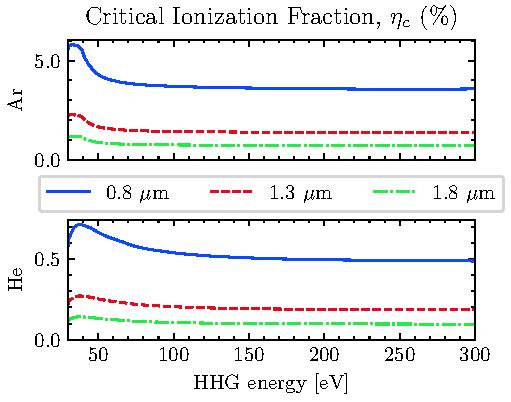
\includegraphics[width=0.75\textwidth]{figures/chap1/crit_ion_frac.pdf}
	\caption{The critical ionization fraction, $\eta_c$ for argon (solid lines) and helium (dashed lines) at different fundamental wavelengths. Refractive index information from \cite{gulliksonCXROXRayInteractions,peckDispersionArgon1964,mansfieldDispersionHelium1969}.}
	\label{fig:crit_ion_frac}
	%figure created using: \Python Scripts\CXRO\test\critical_fraction.py
\end{figure}

\begin{figure}
	\centering
	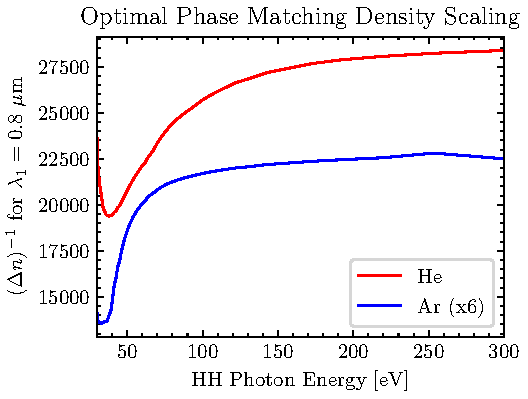
\includegraphics[width=0.75\textwidth]{figures/chap1/recip_deltan_plot.pdf}
	\caption{The optimal phase matching density, $\rho_{opt}$ is inversely proportional to the refractive index mismatch, $\Delta n$. See \cref{eqn:refractive_index_mismatch,eqn:phase_matching_density} for details. As a result, higher interaction pressures are needed to properly phase match higher photon energies. The data shown is for a fundamental wavelength of 800 nm, but the same trend holds for $\lambda_1 = 0.4 - 2.0 \ \mu \textrm{m}$. Refractive index information from \cite{gulliksonCXROXRayInteractions,peckDispersionArgon1964,mansfieldDispersionHelium1969}.}
	\label{fig:recip_deltan_plot}
	%figure created using: \Python Scripts\CXRO\test\critical_fraction.py
\end{figure}

HHG will be an efficient process if the wave vector mismatch $\Delta k$ of the independent dipoles is zero. The phase mismatch term can be expressed as four separate factors, each arising from distinct physical phenomena \cite{rothhardtAbsorptionlimitedPhasematchedHigh2014}:
\begin{equation}
\Delta k \equiv q k_{\omega} - k_{q \omega} = \Delta k_{\textrm{neutral}} + \Delta k_{\textrm{plasma}} + \Delta k_{\textrm{Gouy}} + \Delta k_{\textrm{dipole}}
\label{eqn:phase_mismatch}
\end{equation}
The first two term represents the dispersion from the generating neutral atoms and the electron plasma. In the discussion that follows below, we will use the refractive index $n$ at STP (pressure $P_0$, number density $\rho_0$, temperature $T_0$), where literature values are readily available. We assume that the index scales linearly with the interaction pressure (density). That is, we assume $n(\rho) = (1-\eta)(\rho / \rho_0) n(\rho_0)$, where $\rho$ is the interaction density before any atoms are ionized and $\eta$ is the ionization fraction of the gas medium. For brevity, we will write the index of refraction at STP as $n = n(\rho_0)$. Using this notation, the neutral dispersion mismatch term for an interaction density $\rho$ is:
\begin{align}
\Delta k_{\textrm{neutral}} &= q k_{\textrm{neutral}}(\lambda_1) - k_{\textrm{neutral}}(\lambda_{q}) \nonumber \\
%&= \frac{q}{2 \pi \lambda_1} (1 - \eta) \frac{\rho}{\rho_0}\Delta n
&= \frac{2 \pi q}{\lambda_1} (1-\eta) \frac{\rho}{\rho_0}\Delta n
\label{eqn:deltak_neutral}
\end{align}
where we have used $k(\lambda)= \omega n /c = n / (2 \pi \lambda)$ and defined $\Delta n$ as:
\begin{equation}
\Delta n \equiv n_{\textrm{neutral}}(\lambda_1) - n_{\textrm{neutral}}(\lambda_q)
\label{eqn:refractive_index_mismatch}
\end{equation}
using the notation $\lambda_q \equiv \lambda_1 / q$ for the wavelength of the $q^{th}$ harmonic with frequency $\omega_q \equiv q \omega$ and $\lambda_1$ ($\omega_1)$ for the laser wavelength (frequency). To compute the plasma mismatch term, we start with the refractive index of a plasma:
\begin{align}
n_{\textrm{plasma}}(\omega) &= \sqrt{1 - \frac{\omega_p^2}{\omega^2}} \approx 1 - \frac{\omega_p^2}{2 \omega^2} \\
\omega_p &= \sqrt{\frac{e^2 \rho_e}{\epsilon_0 m_e}}
\end{align}
where $\omega_p$ is the plasma frequency and $\rho_e = \eta \rho$ is the plasma density. Then, the phase mismatch of the plasma is:
\begin{align}
\Delta k_{\textrm{plasma}} &= q k_{\omega_1} - k_{q \omega_1} \nonumber \\
&= \frac{q}{2 \pi \lambda_1} (n_{\textrm{plasma}}(\omega_1) -n_{\textrm{plasma}}(\omega_q) ) \nonumber \\
&= - \frac{1}{4 \pi \lambda_1} \frac{q^2-1}{q} \frac{\omega_p^2}{\omega_1^2} \nonumber \\
&\approx - \frac{q}{4 \pi \lambda_1} \frac{\omega_p^2}{\omega_1^2} \quad \textrm{(for large $q$)} \nonumber \\
&= - q \eta \rho  r_e \lambda_1
% &= - 4 \pi^2 q r_e \rho_e \lambda_1, \quad \textrm{using } r_e = \frac{1}{4 \pi \epsilon_0} \frac{e^2}{m_e c^2} \nonumber \\
% &= - 4 \pi^2 q r_e \eta \rho \lambda_1, \quad \textrm{using } \rho_e = \eta \rho
\end{align}
Where $r_e$ is the classical electron radius:
\begin{equation}
r_e = \frac{1}{4 \pi \epsilon_0} \frac{e^2}{m_e c^2}
\end{equation}
Note that since $\Delta n > 0$ for the wavelengths of interest, we have $\Delta k_{\textrm{plasma}} \le 0$. Adding the two dispersive terms together, we get an expression for the dispersive phase mismatch terms:
\begin{equation}
% \Delta k_{\textrm{neutral}} + \Delta k_{\textrm{plasma}} = \frac{q}{2 \pi \lambda_1} \left( (1-\eta) \frac{\rho}{\rho_0} \Delta n - 8 \pi ^3 r_e \eta \rho \lambda_1^2 \right)
\Delta k_{\textrm{neutral}} + \Delta k_{\textrm{plasma}} = \frac{2 \pi q}{\lambda_1} (1-\eta) \frac{\rho}{\rho_0}\Delta n - q \eta \rho  r_e \lambda_1
\label{eqn:deltak_dispersive}
\end{equation}
Inspection of \cref{eqn:deltak_dispersive} reveals that there exists a \textit{critical ionization fraction} $\eta_c$ for which the dispersive phase terms sum to zero:
\begin{equation}
% \eta_c \equiv \left( 1+ \frac{8 \pi^3 \rho_0 r_e \lambda_1^2}{\Delta n} \right)^{-1}
\eta_c \equiv \left( 1+ \frac{\rho_0 r_e \lambda_1^2}{2 \pi \Delta n} \right)^{-1}
\end{equation}
We can rewrite \cref{eqn:deltak_dispersive} using $\eta_c$:
\begin{equation}
% \Delta k_{\textrm{neutral}} + \Delta k_{\textrm{plasma}} = \frac{q \Delta n}{2 \pi \lambda_1} \frac{\rho}{\rho_0} \left(1 - \frac{\eta}{\eta_c}\right)
\Delta k_{\textrm{neutral}} + \Delta k_{\textrm{plasma}} = \frac{2 \pi q \Delta n}{\lambda_1} \frac{\rho}{\rho_0} \left(1 - \frac{\eta}{\eta_c}\right)
\end{equation}
The critical ionization fraction for helium and argon is shown in \cref{fig:crit_ion_frac}. Note that for $\eta < \eta_c$, the dispersive mismatch term is positive. We will see below that at the IR focus, phase matching ($\Delta k = 0$) is impossible for $\eta > \eta_c$.

The third term of \cref{eqn:phase_mismatch} is the geometrical phase mismatch caused by focusing:
\begin{align}
\Delta k_{\textrm{Gouy}} &= \pdv{z} \left[ q \arctan\left( \frac{2 z}{b_1} \right) - \arctan \left( \frac{2 z}{b_q} \right) \right] \nonumber \\
&= q \frac{2 b_1}{b_1^2 + 4 z^2} - \frac{2 b_q}{b_q^2 + 4 z^2} \nonumber \\
&\approx -(q-1) \frac{2 b_1}{b_1^2 + 4 z^2}
\end{align}
where $b_1 = 2 z_R$ is the confocal parameter and $z_R$ is the Rayleigh range. For the $q^{th}$ harmonic, we assume the nonlinear process obeys a power law $p$ and $b_q = b_1 p /q$ \cite{schounAttosecondHighHarmonicSpectroscopy2015}. Note that $\Delta k_{\textrm{Gouy}}$ is negative for all values of $z$.

The fourth term arises from the intensity-dependent dipole phase acquired during the electron excursion \cite{lewensteinTheoryHighharmonicGeneration1994,balcouGeneralizedPhasematchingConditions1997,salieresCoherenceControlHighOrder1995}:
\begin{equation}
\Delta k_{\textrm{dipole}} = - \alpha_q \pdv{I}{z}
\label{eqn:deltak_atomic}
\end{equation}
The value of $\alpha_q$ depends on the quantum trajectory the electron takes during its excursion. For short trajectories, {$\alpha_q = 2 \times 10^{-14}$ cm\textsuperscript{2}/W} and for long trajectories, {$\alpha_q = 22 \times 10^{-14}$ cm\textsuperscript{2}/W} \cite{kazamiasPressureinducedPhaseMatching2011,balcouQuantumpathAnalysisPhase1999}. The sign of $\Delta k_{\textrm{dipole}}$ is positive (negative) if the gas source is located upstream (downstream) of the focus.

Experimentally, the phase matching can be adjusted by tuning the laser parameters (wavelength $\lambda$, intensity $I$, pulse duration, focal spot size $w_0$), the gas species ($I_p, \ n$ and $k$) and interaction pressure $P$, and the gas location relative to the laser focus ($z$). Additionally, a variable aperture (iris) located just before the generation lens effectively tunes multiple laser parameters simultaneously, and is known colloquially as ``the magic iris trick" \cite{kazamiasHighOrderHarmonic2002}. Because $\Delta k$ is dependent on the harmonic order $q$, it is impossible to perfectly phase match the entire harmonic spectrum simultaneously. As a result, we adjust the phase matching parameters to optimize the useful part of the harmonic spectrum, usually at the expense of the rest of the spectrum.

Also note that the dispersive terms phase can be controlled by tuning the interaction pressure $p$, while the other terms are (to first order) pressure independent. If we place the gas medium at the focus, $\Delta k_{\textrm{dipole}} = 0$, and $\Delta k_{\textrm{Gouy}} = -(q-1) \lambda / (\pi w_0^2)$. In this case, the condition $\Delta k = 0$ can be met by setting to the density to the \textit{optimal phase matching density} $\rho_{\textrm{opt}}$ \cite{rothhardtAbsorptionlimitedPhasematchedHigh2014,pupeikisWaterWindowSoft2020}:
\begin{equation}
\frac{\rho_{\textrm{opt}}}{\rho_0} = \left( \frac{q-1}{q} \right) \frac{2 \lambda^2}{\Delta n w_0^2 \left(1 - \frac{\eta}{\eta_c}\right)}
%\frac{2 \pi^2}{\Delta n} \left( \frac{q-1}{q} \right) \left( \frac{1}{1-\frac{\eta}{\eta_c}} \right) \frac{\lambda^2}{\pi^2 w_0^2 + \left(\frac{z \lambda}{w_0}\right)^2}
\label{eqn:phase_matching_density}
% this equation follows from my notation.
\end{equation}
%\begin{equation}
%p_{opt} = p_0 \frac{\lambda^2}{2 \pi^2 w_0^2 \Delta \delta \left( 1 - \frac{\eta}{\eta_c} \right)}
%\label{eqn:phase_matching_pressure}
%% this equation is from rothhardtAbsorptionlimitedPhasematchedHigh2014
%\end{equation}

We therefore arrive at the conclusion that the optimal phase matching density scales with the square of the fundamental wavelength. Furthermore, tighter focusing (${w_0 \rightarrow 0}$) and higher ionization fractions (${\eta \rightarrow \eta_c}$) require higher densities to achieve good phase matching. Finally, the optimal phase matching density is inversely proportional to the refractive index mismatch, $\Delta n$. This quantity is shown in \cref{fig:recip_deltan_plot} for helium and argon at $\lambda_1 = 800 \ \textrm{nm}$. From this figure, we can see that higher photon energies neccessitate require higher interaction pressures. Therefore, creating bright harmonics at high photon energies from a long wavelength, relatively weak pulse requires significantly higher interaction pressures than low energy harmonics generated with a loosely focused 800 nm pulse. This is the motivation for designing a vacuum system and gas source that can deliver high interaction pressures (see \cref{sec:HHG_gas_sources}).

\subsubsection{XUV Reabsorption}
\label{sec:XUV_reabsorption}

\begin{figure}
	\centering
	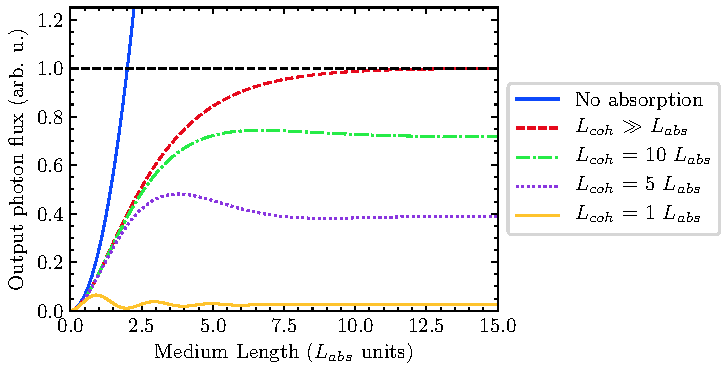
\includegraphics[width=0.75\textwidth]{figures/chap1/Constant1999_fig1.pdf}
	\caption{1D absorption model from \cref{eqn:HHG_Nout_simple}.}
	\label{fig:Constant1999_fig1}
	% created with \Python Scripts\HHG_Phasematching-master\test\Constant_fig1.py
\end{figure}

We now consider the effects of XUV absorption on the phase matching process using the 1-dimension model introduced by Constant et. al. \cite{constantOptimizingHighHarmonic1999}. In doing so, we restrict ourselves to the on-axis emission of the $q$\textsuperscript{th} harmonic. That is, we consider only harmonics with a wave vector $k_q$ that is collinear to the fundamental ($k_0$). In this case, the number of photons emitted per unit time and area is:
\begin{equation}
N_{\textrm{out}} = \frac{\omega_q}{4 c \epsilon_0 \hbar} \left| \left[ \int_{0}^{L_{\textrm{med}}} \dd{z} \rho(z) A_q(z) \exp \left( - \frac{L_{\textrm{med}} - z}{2 L_{\textrm{abs}}}  \right) \exp \left( i \varphi_q(z) \right)  \right] \right|^2
\label{eqn:HHG_Nout}
\end{equation}
Here, $\rho(z)$ is the gas medium density, $A_q(z)$ is the amplitude of the harmonic response at frequency $\omega_q$ and $\varphi_q$ is its phase at the exit of the medium, which has length $L_{\textrm{med}}$. If we are using a loose focusing geometry, then the gas density and harmonic response amplitude are constant along the interaction volume: $\rho(z) = \rho$ and $A_q(z)=A_q$. With this restriction, \cref{eqn:HHG_Nout} evaluates to:
\begin{equation}
\begin{aligned}
N_{\textrm{out}} = & \\ \rho^2 A_q^2 & \frac{4L_{\textrm{abs}}^2}{1+4\pi^2(L_{\textrm{abs}}^2 / L_{\textrm{coh}}^2)} \left[ 1 + \exp\left(-\frac{L_{\textrm{med}}}{L_{\textrm{abs}}}\right) - 2 \exp\left(\frac{\pi L_{\textrm{med}}}{L_{\textrm{coh}}}\right) \exp\left(-\frac{L_{\textrm{med}}}{2L_{\textrm{abs}}}\right) \right]
\label{eqn:HHG_Nout_simple}
\end{aligned}
\end{equation}
Here, we use the notation $L_{\textrm{coh}} = \pi/\Delta k$ for the coherence length ($\Delta k = k_q - q k_0$) and $L_{\textrm{abs}} = 1/{\sigma \rho}$ for the absorption length.

%In the case of no absorption ($L_{\textrm{abs}} \rightarrow \infty$), the harmonic yield grows as $L_{\textrm{med}}^2$.
\cref{eqn:HHG_Nout_simple} is plotted in \cref{fig:Constant1999_fig1}.  In the limit of good phase matching ($L_{\textrm{coh}} \gg L_{\textrm{abs}}$), short interaction length ($L_{\textrm{coh}} \gg L_{\textrm{med}}$) and low absorption ($L_{\textrm{med}} \gg L_{\textrm{abs}}$) the harmonic yield scales as \cite{takahashiGenerationStrongOptical2004}:
\begin{equation}
N_{\textrm{out}} \sim A_q^2 z_0 (\rho L_{\textrm{med}})^2 \sim S_{\textrm{spot}} (P L_{\textrm{med}})^2
\label{eqn:HHG_Nout_2}
\end{equation}
where $z_0 = \pi w_0^2 / \lambda_1$ is the Rayleigh length and $S_{\textrm{spot}} = \pi w_0^2$ is the spot area at the focus. In this limit, the photon yield is proportional to the square of the pressure-length product. Otherwise, the optimized conditions are $L_{\textrm{med}} > 3 L_{\textrm{abs}}$ and $L_{\textrm{coh}} > 5 L_{\textrm{abs}}$.

The dipole strength is assumed to follow $A_q \sim (1-\eta)I_0^5$, where $I_0$ is the intensity at the focus \cite{krauseCalculationPhotoemissionAtoms1992,kuhnELIALPSFacilityNext2017}.

Experimentally, $L_{\textrm{med}}$ is fixed by the geometry of the gas source, $L_{\textrm{abs}}$ is directly controlled by adjusting the backing pressure, and $L_{\textrm{coh}}$ is indirectly controlled by other parameters (gas source position relative to focus, focusing conditions, iris diameter, etc.). In \cref{sec:HHG_gas_sources}, we will apply this simple model to the gas sources available in our lab to maximize our HHG yield.

\textbf{to do:}

motivation: in the LPC, we can't see pressure rollover. this plot helps show why. (assuming the LPC and the free jet are still on the rising edge of the curves). this plot explains why.

talk about choice of generating gas (He vs Ar) in terms of critical ionization fraction and Ip, as well as cross section $A_q$. He, with its low reabsorption, is great for showing interaction pressure scaling, and you can blast it with lots of 800 nm intensity. but overall it has a lower yield than argon b/c of the cross section. Ar performs poorly at 800 nm b/c of the cooper minimum; at longer wavelengths the cutoff extends past the cooper minimum and Ar is a good choice.

\section{IR Beam Shaping Using a Binary Phase Mask}
\label{sec:pi-plate-math}

\begin{figure}
	\centering
	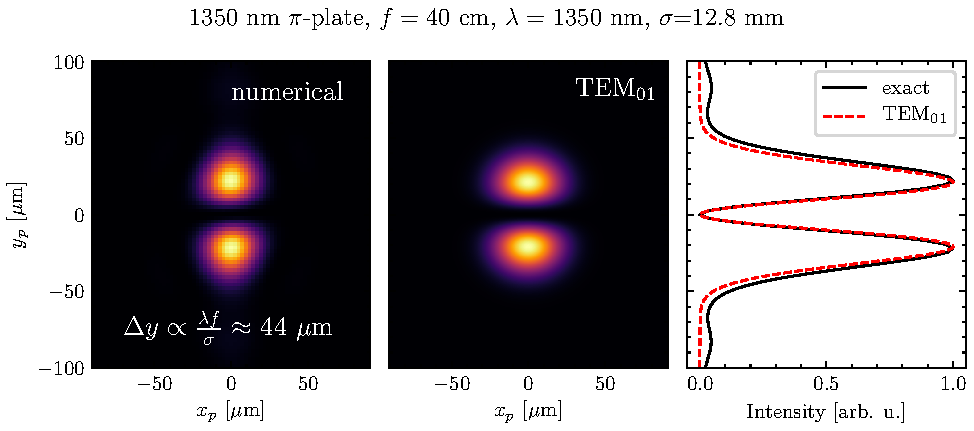
\includegraphics[width=0.75\textwidth]{figures/chap1/pi_plate_focus_LP_TEM_1350nm.pdf}
	\caption{Focus of the IR beam after passing through a centered $\pi$-plate. Left panel: numerical evaluation of the intensity (modulus squared of \cref{eqn:diffraction_integral} using \cref{eqn:fresnel_paraxial_approx}) and a measured input laser beam profile. Middle panel: intensity profile of an equivalent TEM\textsubscript{01} mode. Right panel: intensity lineouts at $x_p = 0$ comparing the numerical result to the TEM\textsubscript{01} mode.}
	\label{fig:pi_plate_focus_sim}
	% \Python Scripts\piplate\piplate_analytical.py
\end{figure}

%\begin{figure}
%	\centering
%	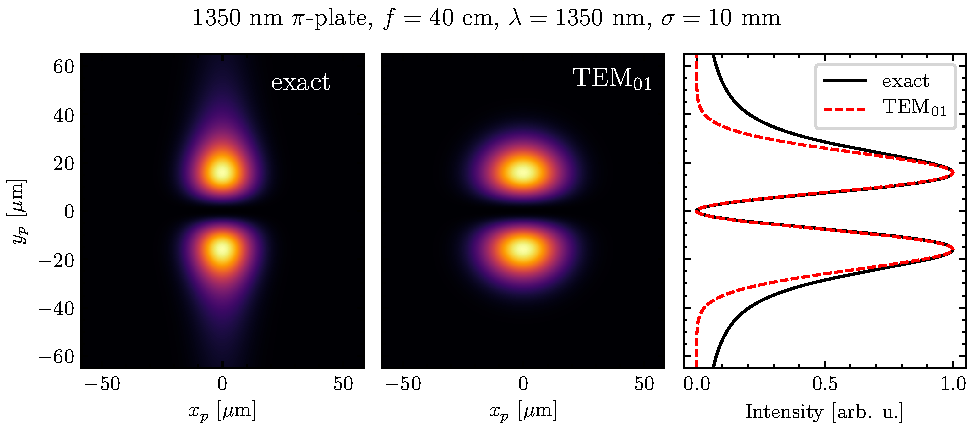
\includegraphics[width=0.75\textwidth]{figures/chap1/pi_plate_focus_sim.pdf}
%	\caption{Simulation of the $\pi$-plate focus, following \cref{eqn:pi-plate-intensity-focus,eqn:TEM01_mode}. Left and middle panels show the exact and approximate intensity profiles at the focus, respectively. The right panel shows intensity lineouts at $x_p=0$.}
%	\label{fig:pi_plate_focus_sim}
%	% \Python Scripts\piplate\piplate.py.
% NOTE: this figure was based on an incorrect analytical solution.
%\end{figure}

In some experiments, we use a phase mask to shape the IR beam profile at the focus. We have used two types of phase masks: a binary phase mask and a phase grating. In this document, we will restrict our discussion to the binary phase mask; see Stephen Hageman's dissertation \cite{hagemanComplexAttosecondTransientAbsorption2020} and \cite{camperHighRelativephasePrecision2019} for details about the phase grating. As will be shown below, a binary phase mask converts a TEM\textsubscript{00} mode into a TEM\textsubscript{01}-like mode at the focus \cite{hagemanComplexAttosecondTransientAbsorption2020,camperHighRelativephasePrecision2019,camperTransverseElectromagneticMode2015,camperHighharmonicPhaseSpectroscopy2014,camperCombinedHighharmonicInterferometries2015}. The two IR spots are phase-locked to each other with a phase difference of $\pi$ (the phase difference is tunable if using a phase grating). If the beam is focused onto a gas plume, each intensity lobe will locally drive HHG, and the harmonics will spatially interfere in the far-field. Below, we will show how a binary phase plate can produce a TEM\textsubscript{01}-like mode at the focus.

The binary phase plate is a planar transmissive optic with a thickness step of size $h$ at its center. Light passing through the thicker half of the plate experiences a phase shift of $\phi$ relative to the light transmitted through the thinner half of the plate:
\begin{equation}
\phi = 2 \pi h (n-1)/\lambda
\end{equation}
where $n$ is the refractive index of the glass. Ignoring Fresnel losses and material absorption, the phase plate has a complex transmittance, $\tau_{pp}$:
\begin{equation}
\tau_{pp} (x, y) =  \begin{cases}
1, & \textrm{for $y > y_0$}.\\
\exp (-i \phi), & \textrm{for $y \le y_0$}.
\end{cases}
\label{eqn:phase-plate-transmission}
\end{equation}
The parameter $y_0$ denotes the position of the phase step relative to the optical axis. We use a plate that has been manufactured with $\phi=\pi$ for $\lambda = 1350 \textrm{ nm}$. Immediately after the phase plate, we place a lens of focal length $f$, which imparts an approximately quadratic phase onto the beam. The complex transmittance of the lens is given by $\tau_L$ \cite{goodmanIntroductionFourierOptics1996}:
\begin{equation}
\tau_L = \exp \left( - \frac{k}{2 f} (x^2 + y^2) \right)
\label{eqn:complex_transmittance_lens}
\end{equation}
We will use scalar diffraction theory to evaluate the electric field at a point $P=(x_p, y_p, z_p)$ located downstream of the phase plate \cite{passillySimpleInterferometricTechnique2005}:
\begin{equation}
E(x_p, y_p, z_p) = \frac{i}{\lambda} \int_{+ \infty}^{- \infty} \int_{+ \infty}^{- \infty} \tau_{L} (x,y) \tau_{pp} (x,y) E_{in} (x,y) \frac{e^{-i k r}}{r} \dd{x} \dd{y}
\label{eqn:diffraction_integral}
\end{equation}
where $E_{in}(x,y)$ is the input electric field at the phase plate and $r$ is the radial coordinate:
$$
r = \sqrt{(x_p-x)^2 + (y_p-y)^2 + z_p^2}.
$$
We apply the Fresnel and the paraxial approximations,
\begin{equation}
\frac{e^{-i k r}}{r} \approx \frac{1}{z_p} \exp \left[-ik \left(z_p + \frac{(x_p-x)^2 + (y_p-y)^2}{2z_p} \right) \right]
\label{eqn:fresnel_paraxial_approx}
\end{equation}
which is valid if $P$ is close to the optical axis. Using this approximation, \cref{eqn:diffraction_integral} was numerically integrated and evaluated at the focus \cite{vdovinLightPipesPython}. $E_{in}$ was calculated by imaging the TOPAS signal beam using a thermal camera and scaling it by the magnification factor of the generation arm's telescope (${M=5/3}$). The resulting intensity at the focal plane is shown in \cref{fig:pi_plate_focus_sim}. We can see that there are two intensity lobes at the focus. The profile is quasi-Gaussian along the $x_p$-direction, and there are maxima located at:
\begin{equation}
y_p \approx \pm \frac{\lambda f}{2 \sigma}
\label{eqn:pi-plate-separation}
\end{equation}
Where $\sigma$ is the beam size of an equivalent Gaussian input beam:
\begin{equation}
E_{in}(x,y) = \exp \left[ - \left( \frac{x^2+y^2}{\sigma^2} \right) \right]
\label{eqn:gaussian_profile}
\end{equation}
%
%The relatively simple form of \cref{eqn:phase-plate-transmission} allows for direct integration of \cref{eqn:diffraction_integral}. Below, we will perform this intergral and evaulate the result at the focus ($z_p = f$). For the general case of a $\pi$-plate ($\phi=\pi$) with an arbitrary offset $y_0$, \cref{eqn:diffraction_integral} evaluates to:
%\begin{equation}
%\begin{aligned}
%E(x_p, y_p, z_p = f; y_0) = \frac{k \sigma^2}{\sqrt{\pi} f} & \exp \left[ - \frac{ik}{2f}(x_p^2+y_p^2+2f^2-2y_0y_p) \right] \times \\
%& \exp \left[ -\left( \frac{k\sigma}{2f} \right)^2 x_p^2 \right] \exp \left[ -\left( \frac{y_0}{\sigma} \right)^2 \right] D \left(-i \frac{y_0}{\sigma} - \frac{k \sigma y_p}{2f} \right)
%\end{aligned}
%\end{equation}
%where $D(x) \equiv \exp(-x^2) \int_{0}^{x} \exp(y^2) \dd{y}$ is the Dawson integral. Note that $D(x)$ is real-valued for real $x$, but complex-valued for complex $x$. Furthermore, $D(x)$ is an odd function with extrema at $x \approx \pm 0.9241$ and $D(0)=0$. We find the intensity by taking the square of the modulus of the electric field:
%\begin{equation}
%\begin{aligned}
%I(x_p, &y_p, z_p = f; y_0) = \\ & \frac{k^2 \sigma^4}{2 \mu_0 c \pi f^2} \exp \left[ - \left( \frac{k \sigma}{\sqrt{2} f} \right) ^2\right] \exp \left[ - \frac{2 y_0^2}{\sigma^2} \right] \left| D \left( - i \frac{y_0}{\sigma} - \frac{k \sigma y_p}{2f}\right) \right|^2
%\end{aligned}
%\end{equation}
%Centering the phase plate on the optical axis ($y_0=0$) gives the desired result. In this case, \cref{eqn:diffraction_integral} evaluates to:
%\begin{equation}
%\begin{aligned}
%E(x_p, &y_p, z_p = f; y_0=0) = \\
%& \frac{k \sigma^2}{\sqrt{\pi}f} \exp \left[ - \frac{ik}{2f} (x_p^2+y_p^2+2f^2)\right] \exp \left[- \left(\frac{k \sigma}{2f}\right)^2 x_p^2 \right] D \left( \frac{k \sigma}{2f} y_p \right)
%\end{aligned}
%\label{eqn:pi-plate-field-focus}
%\end{equation}
%Likewise, the intensity is:
%\begin{equation}
%\begin{aligned}
%I(x_p, y_p, z_p = f; y_0=0) = \frac{k^2 \sigma^4}{2 \mu_0 c \pi f^2} \exp \left[- 2 \left(\frac{k \sigma}{2f}\right)^2 x_p^2 \right] \left| D \left( \frac{k \sigma}{2f} y_p \right) \right|^2
%\end{aligned}
%\label{eqn:pi-plate-intensity-focus}
%\end{equation}
%The intensity has a Gaussian profile along the $x_p$-direction, and there are maxima located at:
%\begin{equation}
%y_p \approx \pm 0.2941 \frac{\lambda f}{\sigma}
%\label{eqn:pi-plate-separation}
%\end{equation}
We therefore see that a TEM\textsubscript{00} beam sent through a centered $\pi$-plate and a lens will have two intensity lobes at the focus. It can be shown that the peak intensity of each lobe is roughly 37\% of the intensity of a TEM\textsubscript{00} mode under identical focusing conditions (ignoring Fresnel losses from the phase plate).
%Inspection of \cref{eqn:pi-plate-field-focus} reveals that the amplitude of the field is even with respect to $x_p$ and odd with respect to $y_p$. Therefore, ${E(x_p, y_p, z_p=f; y_0=0) = - E(x_p, -y_p,  z_p=f; y_0=0)}$, and the phase difference between the two intensity lobes is $\pi$.
This beam profile is very similar to the intensity profile of a TEM\textsubscript{01} mode with an appropriate choice of the beam waist $w_0$:
\begin{align}
I_{01}(x_p,y_p,f) &\propto \frac{8 y_p^2}{w_0^2} \exp\left[- \frac{2(x_p^2+y_p^2)}{w_0^2}\right] \label{eqn:TEM01_mode} \\
\textrm{with} \quad w_0 &\approx \frac{\sqrt{2}}{2} \left( \frac{ \lambda f}{\sigma} \right) \nonumber
\end{align}
For this reason, it is often said that the $\pi$-plate converts a TEM\textsubscript{00} beam into a TEM\textsubscript{01} mode at the focus. The comparison between the numerical and the TEM\textsubscript{01} approximation for a centered $\pi$-plate are shown in \cref{fig:pi_plate_focus_sim}.
